% Document class
\documentclass{paper}
% Commands
\newcommand{\daformula}[0]{\sqrt{D^2 + \left(y - \frac{B + S}{2}\right)^2}}
\newcommand{\dbformula}[0]{\sqrt{D^2 + \left(y + \frac{A + S}{2}\right)^2}}
\date{}
\author{}
% Project metadata

\title{An exploration of the double slit experiment with different width slits and sound waves}
\begin{document} 
\maketitle
\begin{abstract}
    Young's Double Slit experiment is a well known investigation
    in quantum physics, but is traditionally performed using two
    slits of equal width, and uses the small wavelength of light
    to its advantage, e.g. by performing approximations, to yield
    a simple yet reliable theory of interference. This paper 
    attempts to explore the experiment using sound waves,
    that do not have such small wavelengths, and also attempts to 
    generalise the theory further to account for differing slit widths
    rather than restricting itself to two slits of the same width.
\end{abstract}

Word count: 3747 (excluding appendices)

\pagebreak
\tableofcontents
\pagebreak
\section{Wave behaviour}
In this section we introduce two basic characteristics of wave behaviour: \textbf{interference} and \textbf{diffraction}. 
\subsection{Wave interference}
\textbf{Waves} are a simple and useful mathematical concept used by physicists to desribe natural phenomena. Often, we use waves when something is oscillating or periodic, or when it exhibits such behaviours as \textbf{interference} or \textbf{diffraction}. We usually represent e.g. light, sound, etc. as sine waves. Below a sine wave is shown:

\begin{figure}[H]
\caption{A sine wave}
\label{fig:sine-wave}
\begin{tikzpicture}

\draw (0,0) -- (10, 0) node[below, midway]{Time};
\draw (0, -5) -- (0,0);
\draw (0,0) -- (0, 5) node[above,rotate=90, midway]{Displacement};

\draw[domain=0:10, samples=600] plot ({\x}, {5 * sin(\x * 1.2 r)});

\end{tikzpicture}
\end{figure}

The sine wave in \figref{fig:sine-wave} could represent a sound wave, for example. Let us see what happens if we attempt to add two waves. For this text, we will only discuss adding waves of the same wavelength. Below is a figure showing two sine waves (blue and red) that are in phase, and the resultant wave (in green):

\begin{figure}[H]
\label{fig:adding-two-sine-waves}
\caption{Superposition of waves}

\begin{tikzpicture}

\draw (0,0) -- (10, 0) node[midway, below]{Time};
\draw (0, -5) -- (0, 0);
\draw (0,0) --(0, 5) node[above, rotate=90, midway]{Displacement};

\draw[red, domain=1:10, samples=600] plot ({\x}, {sin(\x * 1.2 r)});

\draw[blue, domain=1:10, samples=600] plot ({\x}, {3 * sin(\x * 1.2 r});

\draw[green, domain=1:10, samples=600] plot ({\x}, {4 * sin(\x * 1.2 r});


\end{tikzpicture}

\end{figure}

As we see from the figure above, the two waves have added together to create a bigger wave! This is known as  \textbf{constructive interference}. Of course, if we shift a wave over by a phase shift of $2n\pi, n\in\mathbb{Z}$, or shift it over by a path difference of $n\lambda$, then the wave will be identical. Thus, in order to have constructive interference at any point, we have the criteria

\begin{equation*}
    \Delta x = n\lambda,
\end{equation*}
where $\Delta x$ is the path difference between the two waves.

Note that the phase shift $\phi$ between two waves is given by

\begin{equation}
    \label{eq:path-difference-to-phase-shift}
    \phi = \frac{2\pi}{\lambda}\Delta{x},
\end{equation}
where $\Delta{x}$ is their path difference.
Now, if we shift one wave over by an angle of $\pi$, then the waves will add together to form a smaller wave:

\begin{figure}[H]

\begin{tikzpicture}

\draw (0,0) -- (10, 0) node[midway, below]{Time};
\draw (0, -5) -- (0, 0);
\draw (0,0) --(0, 5) node[above, rotate=90, midway]{Displacement};

\draw[red, domain=1:10, samples=600] plot ({\x}, {sin(\x * 1.2 r)});

\draw[blue, domain=1:10, samples=600] plot ({\x}, {3 * sin(\x * 1.2 r});

\draw[green, domain=1:10, samples=600] plot ({\x}, {sin(\x * 1.2 r) + 3 * sin((\x * 1.2 + pi) r});


\end{tikzpicture}

\end{figure}

In this case, we see that we  end up with a wave with a smaller amplitude once we add the two waves together. If the two waves had the same amplitude, they would completely cancel each other out! This is known as \textbf{destructive interference}.

\subsection{Wave diffraction}
We know from everyday experiences that we can hear around corners, but not see around corners. Why is this? We can explain this using the concept of \textbf{wave diffraction}. Diffraction occurs whenever a wave encounters an obstacle, like a corner. The waves \Quote{bend} around the corners of the obstacle. Below is an image showing water waves diffracting in a ripple tank:

\begin{figure}[H]
    \caption{Water waves diffracting in a ripple tank}
    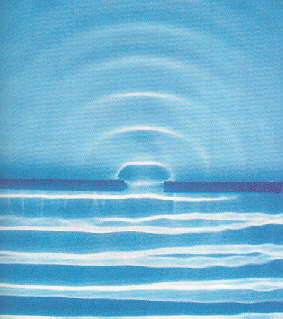
\includegraphics{diagrams/water-wave-diffraction.jpg}
    \source{http://labman.phys.utk.edu/phys222core/modules/m9/images/misc3a.jpg}
\end{figure}

It is known that diffraction only occurs when the width of the obstacle is comparable to the wavelength of the wave.


\section{The standard Double Slit Theory}
\subsection{Zero intensity points}
\label{section:zero-intensity}

One of the most important parts of the standard Double Slit theory is
the formula for finding the points at which the total intensity is zero.
occurs. The formula relies on the fact that the path difference $\Delta{x}$ to any point on
the screen from the two slits can be well approximated by $\Delta{x} = \frac{1}{2}D\sin{\theta}$. (See \figref{fig:double-slit-raw} below)

\begin{figure}[H]
    \caption{Double slit experiment with two slits of equal width}
    \label{fig:double-slit-raw}
    \begin{tikzpicture}
        
        \draw (-0.5, 3.2) -- (-0.5, -3.2);
        \draw (-1.5, 3.2) -- (-1.5, -3.2);
        \draw[<->, very thick] (-0.7, 0) -- (-1.3, 0) node(lambda)[midway, above]{$\bm{\lambda}$};
        
        \draw[<->, very thick] (0,0) -- (10,0) node(D)[midway, above]{$\bm{D}$};
        \draw (10, 5) -- (10, -5);
        
        \draw (0, 1) -- (0, -1);

        \draw (0,5) -- (0 ,3);
        \draw[<->, very thick] (0.5, 2.7) -- (0.5, 1.3) node(b1)[midway, right]{$\bm{b}$};
        
        \draw (0 ,-5) -- (0 ,-3);
        \draw[<->, very thick] (0.5, -2.7) -- (0.5, -1.3) node(b2)[midway, right]{$\bm{b}$};
    
        \draw[->, very thick] (0,0) -- (10,4);
        
         \draw[very thick] (1,0) arc (0:68.2:0.35) node(theta)[midway, xshift=7.5pt, yshift=1.5pt]{$\bm{\theta}$};
        
    \end{tikzpicture}
\end{figure}
The Double Slit Theory relies on the fact that the angle to any given point on the screen from both slits
is approximately the same, because the distance $D$ to the screen is much greater than the distance between
the slits. However, when waves with larger wavelengths, e.g. sound waves, are used, this approximation is no
longer justified. Therefore, this investigation will use a different method, and, as will be see later,
will rely on the widths of the slits and the width of the object separating them instead.
Let $\omega$ be the angular frequency of the waves. By virtue of the relationship $v =                          \lambda\frac{\omega}{2\pi}$,
it is trivial to see that $\omega = 2\pi\frac{v}{\lambda}$, where $v$ is the propagation speed of the waves.
Since the two slits have equal widths, the amplitudes of the waves emitted from both
slits are equal. If the wavelength of the waves used is much larger than the slit widths,
the effects of diffraction will be negligible, and so the superposition $S$ of the two waves can be modelled by 
the equation 
\begin{equation}
    \label{eq:model-superposition-simple}
    S = \sin{\omega{}t} + \sin(\omega{}t + \phi).
\end{equation}
 The phase shift $\phi$ is given
by $\phi = \frac{2\pi}{\lambda}\Delta{x}$, and zero intensity requires $S = 0$ for all $\in\mathbb{R}$,
hence we have 
\begin{equation*}
    \phi = (2n-1)\pi, n\in\mathbb{Z} \implies \frac{1}{2}D\sin{\theta} = \frac{(2n-1)\lambda}{2},
\end{equation*}
which implies 
\begin{equation}
    \label{eq:double-slit-formula}
    D\sin{\theta} = (2n-1)\lambda
\end{equation}
This is the famous \textit{Double Slit Formula}. However, there is an issue,
as the model in \eqref{eq:model-superposition-simple} is a simplification: it does not account for the fact that the path difference of the two slits
to the point will have an impact on the amplitudes of the two waves; the waves emitted
from the slit closer to the point will have a larger amplitude. Of course, when the
experiment is performed with light, this path difference is negligible compared to
the distance to the screen, but when performed with e.g sound waves, it is no longer
negligible, and must be taken into consideration. 

\subsection{Constructive interference}
Another important part of the Double Slit Theory is the position of the
points at which total constructive interference occurs. Modifying the 
\textit{Double Slit Formula} \eqref{eq:double-slit-formula}, we obtain
the condition 
\begin{equation}
    D\sin{\theta} = 2n\lambda.
\end{equation}
However, once again, this formula does not generalise to waves with larger wavelengths
and/or slits with differing widths. Using the formula for the phase shift from \eqref{eq:path-difference-to-phase-shift}
and the condition $\phi = 2n\pi$, we obtain the condition
\begin{equation}
    \label{eq:condition-constructive-interference}
    \lvert{}d_{b} - d_{a}\rvert = n\lambda.
\end{equation}

\section{Finding an expression for the distances from the slits to a given point}
\label{section:distance-formulas}

We will use the \textit{Law of inverse squares} \parencite{inverse-square},
and assume that the amplitude is inversely proportional to the square of the distance
from the source to the screen. Let $d_a$ and $d_b$ be the distances from the slits
to the screen. Let the two slits have widths $A$ and $B.$
The distance from the slits to the screen is $D$. The width of the separator between the slits is $S$,
and the wavelength of the waves is $\lambda$.
(See \figref{fig:double-slit-different-widths} below)

\begin{figure}[H]
\caption{Double slit experiment with two slits of different widths}
\label{fig:double-slit-different-widths}
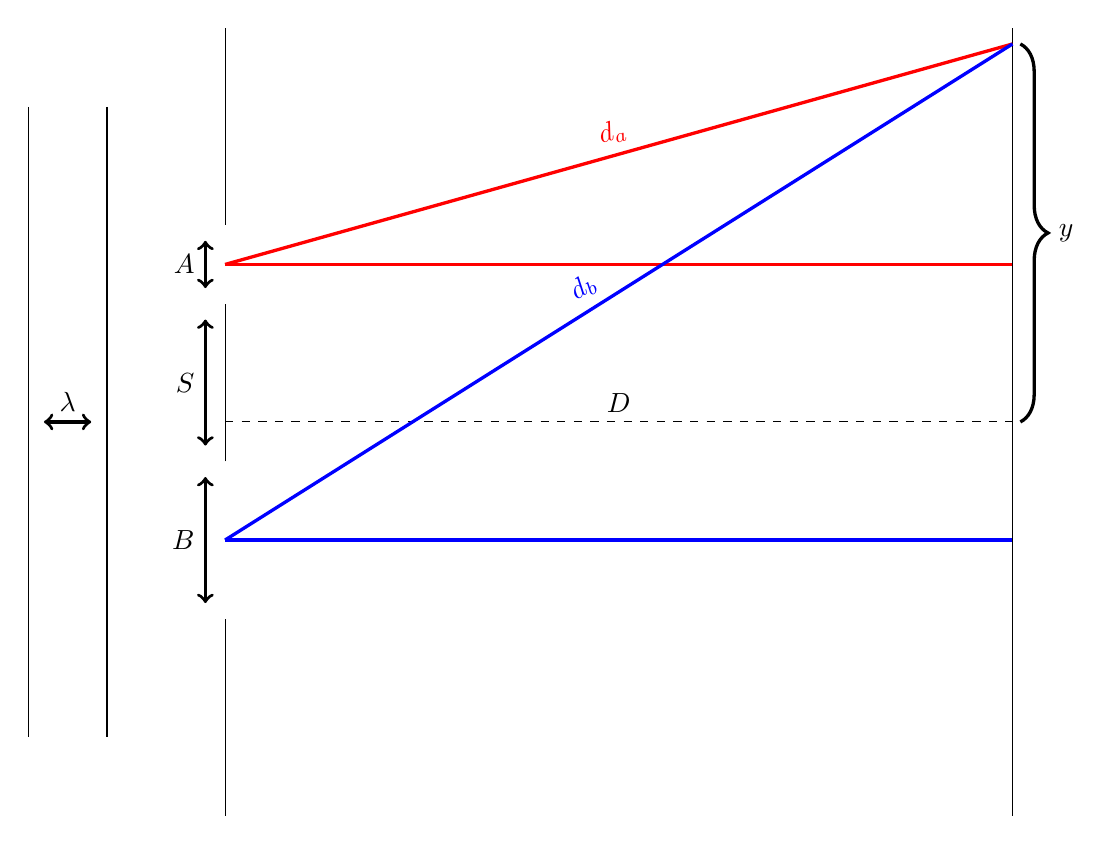
\begin{tikzpicture}

    \draw (-1.5, 4) -- (-1.5, -4);
    \draw (-2.5, 4) -- (-2.5, -4);
    \draw[<->, very thick] (-1.7, 0) -- (-2.3, 0) node(lambda)[midway, above]{$\bm{\lambda}$};

    \draw[dashed] (0,0) -- (10,0) node(D)[midway, above]{$\bm{D}$};

    \draw (10,5) -- (10,-5);
    
    \draw (0,5) -- (0,2.5);
    \draw[<->, very thick] (-0.25, 2.3) -- (-0.25, 1.7) node(A)[midway, left]{$\bm{A}$};
    
    \draw[color=red, very thick] (0,2) -- (10,4.8) node(da)[midway, above, rotate=15.64]{$\bm{d_a}$};
    \draw[color=red, very thick] (0,2) -- (10,2);
    
    \draw (0, -5) -- (0, -2.5);
    \draw[<->, very thick] (-0.25, -0.7) -- (-0.25, -2.3) node(B)[midway, left]{$\bm{B}$};
    
    \draw[color=blue, very thick] (0,-1.5) -- (10, -1.5);
    \draw[color=blue, very thick] (0,-1.5) -- (10,4.8) node(db)[midway, above, rotate=32.2, xshift=-10pt]{$\bm{d_b}$};

    \draw[very thick,decorate, decoration={brace, amplitude=10pt}] (10.1, 4.8) -- (10.1, 0) node(y)[midway, right, xshift=10pt]{$\bm{y}$};


    \draw (0,-0.5) -- (0,1.5);
    \draw[<->, very thick] (-0.25,-0.3) -- (-0.25, 1.3) node(S)[midway, left]{$\bm{S}$};
\end{tikzpicture}
\end{figure}

The dashed line in \figref{fig:double-slit-different-widths} above
defines the points that are equidistant from the bottom of slit $A$ and the top of slit $B$
as seen in the diagram. The distance from the top of slit $A$ to the bottom of slit $B$ is
Then, the model in \eqref{eq:model-superposition-simple}
becomes 
\begin{equation}
    S = \frac{1}{d_{a}^{2}}\sin{\omega{}t} + \frac{1}{d_{b}^{2}}\sin(\omega{}t + \phi),
\end{equation}
Now, we must take into account that the two slits may not be same width. We will
assume that the amplitude of the waves emitted from the slits is proportional to the width of the slits.
For justification, note that a slit twice as large will collect twice as much sound, light, etc.
Let the two slits have widths $A$ and $B$ respectively, and the model becomes
\begin{equation}
    S = \frac{A}{d_{a}^{2}}\sin{\omega{}t} + \frac{B}{d_{b}^{2}}\sin(\omega{}t + \phi).
\end{equation}

The distance from the top of slit $A$ to the bottom of slit $B$ is given by

\begin{equation*}
    A + B + S.
\end{equation*}

Therefore, the distance from the top of slit $A$ to the midpoint of the two slits is

\begin{equation}
\label{eq:distance-from-slit-A-to-midpoint}
    \frac{A + B + S}{2}.
\end{equation}

Subtracting the distance from the top of slit $A$ to the middle of slit $A$ ($\frac{A}{2}$)
gives the distance from the middle of slit $A$ to the midpoint of the two slits:

\begin{equation*}
    \frac{A + B + S}{2} - \frac{A}{2} = \frac{B + S}{2}.
\end{equation*}

Subtracting the above from $y$ gives the length of one of the sides of the red triangle, the other
having length $D$. Hence, $d_a$ is given by 

\begin{equation}
    \label{eq:d_a}
    d_a = \daformula.
\end{equation}

The distance from slit $B$ to the point can be found likewise, but adding instead of subtracting:
            
\begin{equation}
    \label{eq:d_b}
    d_b = \dbformula.
\end{equation}
            
\section{Finding an expression for the phase shift at a given point}

If the path difference $\Delta{x}$ of two waves and their wavelength $\lambda$ is known, it easy to find their
phase shift:
            
\begin{equation*}
    \phi = \frac{2\pi}{\lambda}\Delta{x}.
\end{equation*}
            
In the last section, the distances $d_a$ and $d_b$ from the slits $A$ and $B$, respectively,
to a given point were found. Then, the path difference is simply given by
            
\begin{equation*}
    \Delta{x} = \lvert{}d_b - d_a\rvert{},
\end{equation*}
            
which, when incorporating the results from \eqref{eq:d_a} and \eqref{eq:d_b}, yields
\begin{equation*}
    \Delta{x} = \left\lvert \dbformula - \daformula \right\rvert
\end{equation*}
            
Then, using the formula from \eqref{eq:path-difference-to-phase-shift}, we obtain
            
\begin{equation}
    \label{eq:phase-shift}
    \phi = \frac{2\pi}{\lambda}\left\lvert\ \dbformula - \daformula \right\rvert
\end{equation}
            
\section{Generalised formula for the intensity at any point}
\label{section:intensity-formula}

It would certainly be interesting to derive a formula for the intensity at any given point.
To obtain the total intensity, we will add the amplitudes contributed by
both slits, and square the total amplitude. Since intensity is proportional to the
square of amplitude, and we are only interested in relative/arbitrary units, this is a
legitimate method of obtaining the intensity.
            
    
The amplitude coming from the slit with width $A$ a distance $d_a$ away from the point
will contribute a wave
            
\begin{equation*}
    wave_{a} = \frac{A}{d_{a}^{2}}\sin{\omega{}t}.
\end{equation*}
            
Likewise, the other slit, with a width of $B$ a distance $d_{b}$ away from the point
will contribute a wave 
            
\begin{equation*}
    wave_{b} = \frac{B}{d_{b}^{2}}\sin(\omega{}t + \phi).
\end{equation*}
            
So, adding them together, the superposition $S$ is given by
            
\begin{equation}
\label{eq:S-of-t}
    S = \frac{A}{d_{a}^{2}}\sin{\omega{}t} + \frac{B}{d_{b}^{2}}\sin(\omega{}t + \phi).
\end{equation}
    
Consider a wave that is a sum of waves of the same wavelength and phase. If we double the amplitude of the wave, then the particles' displacement will change \textbf{twice} as quickly, and thus, the wave's energy will change \textbf{four} times as quickly. Then, trivially, it will also change four times as quickly on average, and thus the intensity has quadrupled. So, we say that a wave's intensity is proportional to the square of its amplitude. The core of the argument is that the wave's \textbf{rate of change of energy} is proportional to the square of its \textbf{displacement}, and thus the intensity is proportional to the \textbf{average} if the square of the displacement of the wave. If all the parts of the wave are in phase, we can extend that and say that intensity is proportional to the amplitude of the wave since the square amplitude will indeed be proportional to the average square displacement.

Now, consider a wave that is the sum of waves of the same wavelength but \textbf{different phase}. Then, we use the same argument: The rate of change of energy will be proportional to the particles' displacement. Then,
            

Squaring the above expression in \eqref{eq:S-of-t} gives the rate of change of energy $I(t)$ at a given point at a specific time:
            
\begin{equation}
    \label{eq:superposition-intensity}
    I(t) = \left(\frac{A}{d_{a}^{2}}\sin{\omega{}t} + \frac{B}{d_{b}^{2}}\sin(\omega{}t + \phi)\right)^{2}.
\end{equation}

Notice, however, that $I(t)$ seems to vary with time. So, we will find the average intensity $I$
over one full period. During one period, $\omega{}t$ goes from $0$ to $2\pi$.
Therefore, $t$ goes from $0$ to $\frac{2\pi}{\omega}$, and hence, we need to find the average
intensity with respect to time over the interval $\left[0, \frac{2\pi}{\omega}\right]$. The average
value of some function $f$ over some interval $[x_{0}, x_{1}]$ can be calculated by dividing the
area under the curve on that interval by the length of the interval.
So, the intensity at a given point will be given by

\begin{equation}
    \label{eq:intensity-integral}
    I = \frac{\omega}{2\pi}\int_{0}^{2\pi/\omega}\left(\frac{A}{d_{a}^{2}}\sin{\omega{}t} 
    + \frac{B}{d_{b}^{2}}\sin(\omega{}t + \phi)\right)^{2} \; dt.
\end{equation}

This integral is evaluated in \textbf{\hyperref[appendix:intensity-integral]{Appendix B}}.

Now, using the derivation from \textbf{\hyperref[appendix:intensity-integral]{Appendix B}}, we obtain the following expression for the intensity:
\begin{flalign*}
    \begin{aligned}
    &\quad{}I = \frac{\omega}{2\pi}\left[\frac{A^2}{d_a^4}\times\frac{\pi}{\omega}
        + \frac{2AB}{d_{a}^{2}d_{b}^{2}}\times\frac{\pi}{\omega}\cos{\phi}
        + \frac{B^2}{d_b^4}\times\frac{\pi}{\omega}\right] \\
    &= \frac{1}{2}\left[\frac{A^2}{d_a^4} + 
        \frac{2AB}{d_{a}^{2}d_{b}^{2}}\cos{\phi} + \frac{B^2}{d_b^4}\right].
    \end{aligned}
\end{flalign*}
                
However, since we are using arbitrary units, the factor of $\frac{1}{2}$ is of
no importance, so we can obtain the formula

\begin{equation*}
    I = \frac{A^2}{d_a^4} + 
    \frac{2AB}{d_{a}^{2}d_{b}^{2}}\cos{\phi} + \frac{B^2}{d_b^4}.
\end{equation*}

However, this assumes that the waves are formed at the slits. In reality,
the waves are formed first at the source, and then reformed at the slits due
to diffraction. Let the perpendicular distance from the source to the slits be $k$. 
Then, assuming the waves had an initial amplitude $A_{initial}$
at the source, once they reach the slits, they will have an amplitude $\frac{A_{initial}}{k^2}$,
due to the \textit{Law of Inverse Squares} \parencite{inverse-square}.
Incorporating this into the expression for intensity above gives

\begin{equation}
\label{eq:expression-for-intensity}
    I = \frac{1}{k^2}\left(\frac{A^2}{d_a^4} + 
    \frac{2AB}{d_{a}^{2}d_{b}^{2}}\cos{\phi} + \frac{B^2}{d_b^4}\right).
\end{equation}

\section{Comparing the theory to experimental results}

To test the theory, sound waves were used. It was expected that the theory
would fit the experimental well when the wavelength used was much larger than
the slit widths (corresponding to a low frequency), and that they would not agree
very well when the wavelength used was not much larger than the slit widths.

\subsection{The experiment}
                
A single speaker was placed in a classroom, a distance $k$ away from a doorway of width $87.5$ cm.
In practice, $k$ was never varied; it was kept constant at $244$ cm. (A $1$ metre ruler was used for all distance measurements) A tall (taller than the doorway) piece of cardboard was used to define the slits. It was approximately $9$ cm wide. By placing the
cardboard such that its centre was in the centre of the doorway, two slits of equal width could be
produced; moving it to the left or to the right would make one slit larger than the other;
single slit experiments were performed by not using the cardboard at all. Unfortunately, it was difficult
to find a suitable location for the experiment that allowed for a screen like in the model. Instead, the
sound intensity was measured at a distance of $248$ cm from the doorway. The first measurement was done
$192$ cm \enquote{to the right} of the midpoint, and measurements were made all the way to the midpoint,
and then all the way to the point $192$ cm \enquote{to the left} of the midpoint. On the floor, there were
small white circular dots, with a spacing of $24$ cm. This made it easy to measure the intensity at intervals
of $24$ cm. Using the relationship $v = \lambda{}f \implies f = \frac{v}{\lambda}$, where $v = \SI{340}{\m\per\square\s}$, 
it was trivial to calculate which frequency of sound to use. Once the frequency had been determined,
an online tone generator \parencite{tone-generator} was used to send monochromatic
(only one wavelength) sound waves through the doorway. A mobile app \parencite{sound-meter} was used to record the sound
intensity. However, the mobile app used gave values in dB. According to \parencite{decibel-to-intensity}, $\beta$ dB
is equivalent to an intensity $I$ by the following equation:

\begin{equation*}
    \beta = 10\log_{10}\frac{I}{I_0},
\end{equation*}
                
where $I_0$, the \enquote{standard threshold of hearing} is equal to \SI{10e-12}{\watt\per\square\m} \parencite{decibel-to-intensity}.
Solving for $I$ yields

\begin{equation}
\label{eq:intensity-to-decibel}
    I = I_{0} \times 10^{\frac{\beta}{10}}
\end{equation}

The measured dB values were converted to watts per square metre using the formula above,
and then plotted against the distance from the midpoint. They were then normalised by dividing each
intensity value by the maximum. For each measured value, a predicted value (according to the formula in 
\eqref{eq:expression-for-intensity}) was generated, and a graph was plotted from these values as well.
Once again, the predicted values were normalised. The recorded dB values and their value after conversion to
SI units were also recorded, along with the dB and SI values predicted, in a text file. The code used
to evaluate the intensity formula in \eqref{eq:expression-for-intensity} from \sectionref{section:intensity-formula} is given in \textbf{\hyperref[appendix:diffraction-free-code]{Appendix A.1}}

\subsection{Experimental results}
\label{section:experimental-results}
Six cases in particular were tested. One single-slit experiment, one double-slit
experiment with two slits of equal widths, and one experiment where one slit was twice
as wide as the other. For two of these cases, the experiment was performed first with
a wavelength approximately as large as the largest slit, and afterwards with a wavelength much
larger than the largest slit width. The third case was only investigated with a large wavelength.

\subsubsection{Graphs}
\sectionparagraph{One slit}
Below is a plot of the predicted results vs. the measured results for a small wavelength:

\begin{figure}[H]
\label{fig:single-slit-small-lambda}
\caption{Single slit - Small wavelength}    
    \includegraphics{single-slit-small-lambda}

\end{figure}
From the figure above, it can be seen that the theory does not fit the data.
Now, let us compare theory and results when the wavelength is large:

\begin{figure}[H]
\label{fig:single-slit-large-lambda}
\caption{Single slit - Large wavelength}
    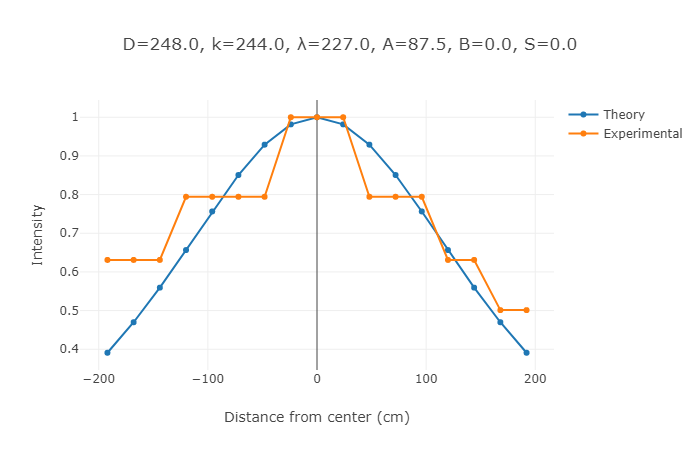
\includegraphics{single-slit-large-lambda}
\end{figure} 

Clearly, in this case, the theory fit the measurements much better.

\sectionparagraph{Two slits of equal width}
Below is a plot of the predicted results vs. the measured results for a small wavelength:

\begin{figure}[H]
\label{fig:double-slit-small-lambda}
\caption{Double slit - Small wavelength}
    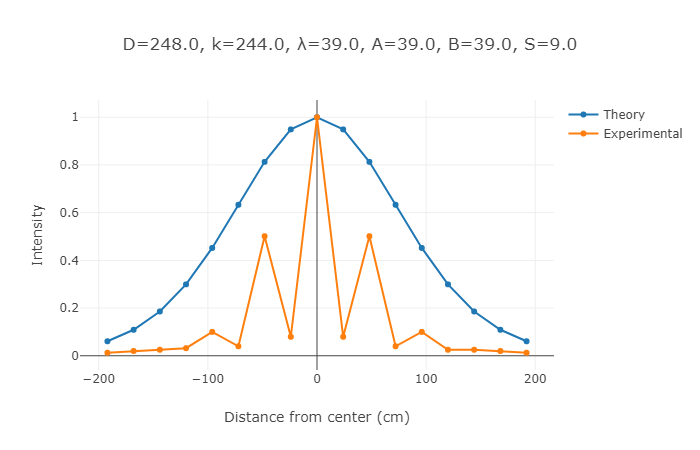
\includegraphics{double-slit-small-lambda}
\end{figure}

We can see that the theory most certainly does not fit the data.
Now, let us compare the results for a large wavelength:

\begin{figure}[H]
\label{fig:double-slit-large-lambda}
\caption{Double slit - Large wavelength}
    \includegraphics{double-slit-large-lambda}
\end{figure}

Once again, the theory is a much better fit when the wavelength is
large.

\sectionparagraph{One slit twice as wide as the other}
Below are the results measured and the predicted results from the theory
for two slits where one is twice as wide as the other:

\begin{figure}[H]
\label{fig:1-2-ratio-large-lambda}
\caption{One slit twice as wide as the other - Large wavelength}
    \includegraphics{1-2-ratio-large-lambda}
\end{figure}

Once again, the theory fits the data well.
In \sectionref{section:zero-intensity}, we said that the theory we have now developed
would only provide an accurate description of the intensity curve if the wavelength was large because
then the effects of diffraction would be negligible.
The results above seem to support this.

\section{Accounting for diffraction}
\label{section:accounting-for-diffraction}

The intensity formula from \eqref{eq:expression-for-intensity} derived in \sectionref{section:intensity-formula} only accounts for interference between the waves. It assumes the waves travel as plane waves from the source to the slits, and then spread out like a point source at the slits. In fact, as long as the wavelength is as large or larger than the slit widths, then there will be a diffraction pattern as well. As discussed in \sectionref{section:intensity-formula}, if the wavelength is much larger than the slit widths, the effects of diffraction can be ignored. We will not attempt to extend our theory to account for diffraction as well, in hopes that a diffraction-including model will agree with the experimental data also for small wavelengths.

Huygen’s principle \parencite{huygens-principle} states that to explain diffraction, we may assume that when a wave undergoes diffraction, every point on the wavefront
acts as a circular point source; so there will be infinitely many circular point
sources. To obtain an expression for the effect on intensity accounting for diffraction, we will assume that at the slits, the wave splits into n point sources, and let n go
to infinity.

Let $I_0$ be the amplitude of the wave as it enters the slits. Since we are using relative units, we will let $I_0 = 1$ for simplicity. We will assume that the amplitude $1$ will be spread evenly across the $n$ point sources; then, each source will have amplitude $\frac{1}{n}$. The distance from the $i$th slit from slit $A$ to the point will be some distance $d_a(i)$, and for slit $B$ we will have a similar expression $d_b(i)$. Because $d_a(i)$ and $d_b(i)$ both will depend on $i$, there will be a specific phase shift for each of the sources. It does not make sense to talk about a \Quote{phase shift} if we do not have a reference source. Arbitrarily, we choose the source in the middle of the slits to be the \Quote{in phase}, and call it the $0$th slit, and assign phase shifts $\phi_a(i)$ and $\phi_b(i)$, respectively, to the other point sources. The top slit will be the \Quote{$-\frac{n - 1}{2}$th} slit, i.e it will have $i = -\frac{n - 1}{2}$, and the bottom slit will be the $\frac{n - 1}{2}$th slit. Below we derive the resultant wave coming from slit $A$ at a given point, and then it will be easy to duplicate the derivation for slit $B$.

The wave $\Lambda_i$ coming from the $i$th source from slit $A$ will be given by

\begin{equation*}
    \Lambda_i = \frac{1}{n \times d_a^2(i)}\sin(\omega t + \phi_a(i)).
\end{equation*}

The resultant wave $\Lambda(n)$, written as a function of $n$, coming from slit $A$ is given by the sum of these waves:

\begin{equation}
    \label{eq:sum-of-sine-waves}
    \Lambda(n) = \sum_{i = -\frac{n - 1}{2}}^{\frac{n - 1}{2}} \frac{1}{n \times d_a^2(i)} \sin(\omega t + \phi_a(i)).
\end{equation}


Next, we will attempt to derive expressions for $d_a(i)$ and $\phi_a(i)$.

\subsection{Deriving expressions for $d_a(i)$ and $\phi_a(i)$}

Recall the diagram from \figref{fig:double-slit-different-widths}:

\begin{figure}[H]
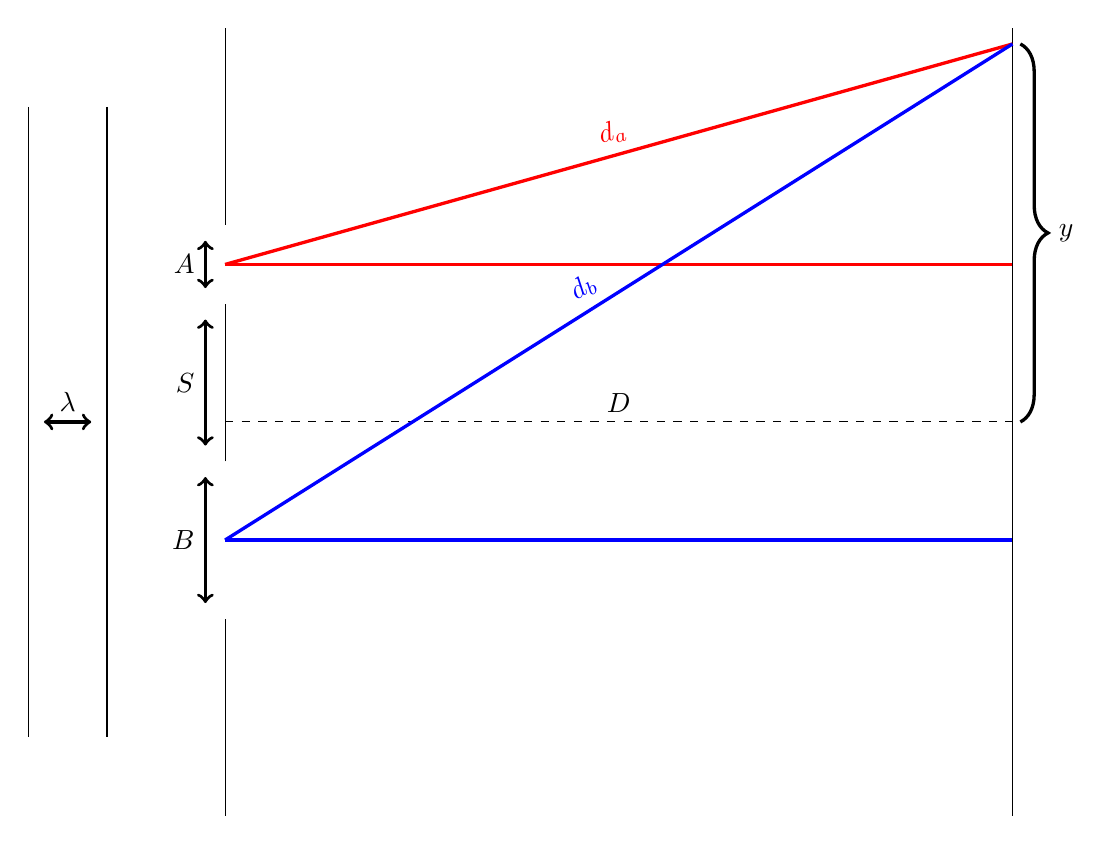
\begin{tikzpicture}

    \draw (-1.5, 4) -- (-1.5, -4);
    \draw (-2.5, 4) -- (-2.5, -4);
    \draw[<->, very thick] (-1.7, 0) -- (-2.3, 0) node(lambda)[midway, above]{$\bm{\lambda}$};

    \draw[dashed] (0,0) -- (10,0) node(D)[midway, above]{$\bm{D}$};

    \draw (10,5) -- (10,-5);
    
    \draw (0,5) -- (0,2.5);
    \draw[<->, very thick] (-0.25, 2.3) -- (-0.25, 1.7) node(A)[midway, left]{$\bm{A}$};
    
    \draw[color=red, very thick] (0,2) -- (10,4.8) node(da)[midway, above, rotate=15.64]{$\bm{d_a}$};
    \draw[color=red, very thick] (0,2) -- (10,2);
    
    \draw (0, -5) -- (0, -2.5);
    \draw[<->, very thick] (-0.25, -0.7) -- (-0.25, -2.3) node(B)[midway, left]{$\bm{B}$};
    
    \draw[color=blue, very thick] (0,-1.5) -- (10, -1.5);
    \draw[color=blue, very thick] (0,-1.5) -- (10,4.8) node(db)[midway, above, rotate=32.2, xshift=-10pt]{$\bm{d_b}$};

    \draw[very thick,decorate, decoration={brace, amplitude=10pt}] (10.1, 4.8) -- (10.1, 0) node(y)[midway, right, xshift=10pt]{$\bm{y}$};


    \draw (0,-0.5) -- (0,1.5);
    \draw[<->, very thick] (-0.25,-0.3) -- (-0.25, 1.3) node(S)[midway, left]{$\bm{S}$};
\end{tikzpicture}
\end{figure}

Straight away, we have $d_a(0) = d_a$, and we know from \eqref{eq:d_a} that $d_a$ is given by

\begin{equation*}
    d_a = \sqrt{D^2 + \left(y - \frac{B + S}{2}\right)^2}.
\end{equation*}

Here, $D$ is the horizontal component of the distance, and $y - \frac{B + S}{2}$ is the vertical component. At the $i$th source, the vertical distance will be $y - \frac{B + S}{2} + \frac{iA}{n - 1}$. To verify this, plug in $i = \frac{n - 1}{2}$, and we get a vertical distance of $\frac{A + B + S}{2}$, which we from \eqref{eq:distance-from-slit-A-to-midpoint} in  \sectionref{section:distance-formulas} know is the distance from the middle of slit $A$ to the midpoint. Since the extra bit ($\frac{iA}{n - 1}$) is proportional to $i$ as well, this is the correct expression to add on.

Thus, $d_a(i)$ is given by

\begin{equation}
    \label{eq:d_a(i)}
    d_a(i) = \sqrt{D^2 + \left(y + \frac{iA}{n - 1} - \frac{B + S}{2}\right)^2}.
\end{equation}

Then, the path difference $\Delta{x}_i$, using source $0$ as a reference, is given by

\begin{equation*}
    \Delta{x}_i = \left\lvert \sqrt{D^2 + \left(y - \frac{B + S}{2}\right)^2} - \sqrt{D^2 + \left(y + \frac{iA}{n - 1} + \frac{B + S}{2}\right)^2} \right\rvert.
\end{equation*}

And the phase shift $\phi_a(i)$ must then be given by

\begin{equation}
    \label{eq:phi_a(i)}
    \phi_a(i) = \frac{2\pi}{\lambda}\left\lvert \sqrt{D^2 + \left(y - \frac{B + S}{2}\right)^2} - \sqrt{D^2 + \left(y + \frac{iA}{n - 1} + \frac{B + S}{2}\right)^2} \right\rvert.
\end{equation}

\subsection{Further derivation}

Using the fact that $\phi = \frac{2\pi}{\lambda}\Delta{x}$, and the formula from \eqref{eq:sum-of-sine-waves}, we have

\begin{equation*}
    \Lambda(n) = \sum_{i = -\frac{n - 1}{2}}^{\frac{n - 1}{2}} \frac{1}{n \times d_a^2(i)} \sin\left(\omega t + \frac{2\pi}{\lambda}(d_a - d_a(i))\right)
\end{equation*}

Notice we are not taking the absolute value of $d_a - d_a(i)$. This is intentional: A certain source above the middle source might be just as much out of phase as a certain slit below the middle, but they would be out of phase in opposite directions. Therefore, we account for this by considering the sign of the path difference.

We will now take the limit as $n$ goes to infinity, yielding the actual resultant wave $\Lambda$ from slit $A$:

\begin{equation*}
    \Lambda = \lim_{n \to \infty} \sum_{i = -\frac{n - 1}{2}}^{\frac{n - 1}{2}} \frac{1}{n \times d_a^2(i)} \sin\left(\omega t + \frac{2\pi}{\lambda}(d_a - d_a(i))\right).
\end{equation*}

Using precisely the same argument for slit $B$, we have the following expression for the resultant wave $\beta$ coming from slit $B$:

Since $n$ is constant with respect to $i$, we can move it outside the summation:

\begin{equation*}
        \Lambda = \lim_{n \to \infty} \frac{1}{n}\sum_{i = -\frac{n - 1}{2}}^{\frac{n - 1}{2}} \frac{1}{ d_a^2(i)} \sin\left(\omega t + \frac{2\pi}{\lambda}(d_a - d_a(i))\right).
\end{equation*}

\begin{equation*}
    \beta = \lim_{n \to \infty} \frac{1}{n}\sum_{i = -\frac{n - 1}{2}}^{\frac{n - 1}{2}} \frac{1}{d_b^2(i)} \sin\left(\omega t + \frac{2\pi}{\lambda}(d_a - d_a(i))\right).
\end{equation*}

Then, the superposition $S$ is given by

\begin{equation*}
    S = \Lambda + \beta.
\end{equation*}

We notice that displacement $S$ of the resultant wave will be a function of $t$. To find the intensity, we will integrate the square of $S$ from $0$ to $2\pi / \omega$ with respect to $t$ and divide by $2\pi / \omega$:

\begin{equation*}
    I = \frac{\omega}{2\pi}\int_{0}^{2\pi / \omega} (\Lambda + \beta) \; dt.
\end{equation*}

The Python code used to evaluate this integral is given in \textbf{\hyperref[appendix:diffraction-code]{Appendix A.2}}
\section{Evaluation}

\subsection{Evaluation of experimental results}
\label{section:precision-and-bias}
Unfortunately, it has to be admitted that the results below most likely suffer from a severe case of confirmation bias and bad precision. There was a lot of background noise (construction work) present during the measurements, and there was never a time when the intensity reading \Quote{settled} properly; the reading was fluctuating with a range of a few decibel. A fluctuation of a few decibel is in fact crushing when it is considered that the decibel difference between each consecutive measurement is also only a few decibel. When the experiment was conducted, the rough shape of double-slit and single-slit curves was known. So, when a choice had to be made whether the reading was e.g $61$, $62$, $63$, or $64$ dB (not actual values), I would be more likely to choose the reading that, relative to the previous readings so far in the trial, would best conform to the known shape. I also knew in advance what curve my model predicted. I knew that it didn't include any maxima or minima except the central maxima. Thinking my model \textbf{should} be correct for large wavelengths, I might have ignored maxima or minima that were actually there. Or, conversely, during the trials with small wavelengths, I knew that there \Quote{were supposed to be other maxima/minima}, and so I would be prone to exaggerating increases or decreases in intensity. In hindsight, it would likely have been a better idea to collect experimental data first, and only then start working on the model. The reader will probably be surprised at how \Quote{nice} the curves with small wavelengths look; This could be explained by the narrow range of values and confirmation bias.

Let us say two points have decibel readings $\beta_1$ and $\beta_2$ which correspond to actual intensities $I_1$ and $I_2$ respectively. Let $I_2 / I_1 = a$. Then, using the formula for decibels from \eqref{eq:intensity-to-decibel}, we have

\begin{equation*}
    \frac{I_1}{I_2} = a \implies \frac{\cancel{I_0} \times 10^{\beta_1 / 10}}{\cancel{I_0} \times 10^{\beta_2 / 10}} = a.
\end{equation*}

Solving for $\lvert \beta_1 - \beta_2\rvert$, the decibel difference, we get

\begin{equation*}
    \lvert \beta_1 - \beta_2 \rvert = \lvert 10\log a \rvert.
\end{equation*}

In the first plot from \sectionref{section:experimental-results}, the central maximum has a relative intensity $1$, and the first maximum to the right has an intensity $0.4$. So, the ratio of these, using $I_1 = 1, I_2 = 0.4$, is
$5/2$. Then, we get

\begin{equation*}
    \lvert \beta_1 - \beta_2 \rvert \approx 4 \; \textnormal{dB}.
\end{equation*}

So, if both readings were off by $2$ dB, this would be within the margin of error. Thus, it is feasible that the maxima/minima were not really there.

\subsection{Evaluation of the diffraction-including model}

For all five of the trials conducted (see \sectionref{section:experimental-results}), the diffraction-including model gave very similar predictions to those of the diffraction-free-model from \sectionref{section:intensity-formula}. The plots are included in \textbf{\hyperref[appendix:diffraction-plots]{Appendix C}}.

This was unexpected. As discussed earlier in the paper, we said that the diffraction-free model did not adhere to the experimental results for small wavelengths because of diffraction. But now we have a model that accounts for diffraction, and it predicts almost the same intensity distribution! Thus, we have two options:

\begin{boldenumerate}
    \item The diffraction-including model is wrong. Either we applied Huygen's principle incorrectly, there is an error in the mathematics somewhere, or the code is wrong.
    
    \item The measurements are incorrect.
\end{boldenumerate}

It is of course possible that the model is wrong. Consider also, though, the discussion of the reliability of the experimental results above. It is possible that there really were no maxima or minima except the central maxima during the trials with small wavelengths, but since I knew in advance that there \Quote{were supposed to be some}, my bias combined with the fluctuation of the readings lead the data to show them.

\pagebreak

\printbibliography[heading=bibintoc]

\pagebreak

\begin{appendices}

\section{Code for computer simulations}
\subsection{Code for diffraction-free model}
\label{appendix:diffraction-free-code}
\pagenumbering{arabic}
\renewcommand*{\thepage}{A\arabic{page}}
\renewcommand{\theequation}{A.\arabic{equation}}
\setcounter{equation}{0}
Below is the code used to check the diffraction-free model from \sectionref{section:intensity-formula} against experimental data.
\lstinputlisting[language=Python,  breaklines=true]{programs/compare-experiment-to-model.py}

\subsection{Code for diffraction-including model}
\label{appendix:diffraction-code}
Below is the code used to visualise the diffraction-including model from \sectionref{section:accounting-for-diffraction}.

\lstinputlisting[language=Python, breaklines=true]{programs/numerical-sums.py}

\section{Evaluation of intensity integral}

\pagenumbering{arabic}
\label{appendix:intensity-integral}
\setcounter{equation}{0}
\renewcommand*{\thepage}{B\arabic{page}}
\renewcommand{\theequation}{B.\arabic{equation}}


Below we evaluate the three integrals from \eqref{eq:intensity-integral} in \sectionref{section:intensity-formula}:

\begin{align}
    \begin{aligned}
    \label{eq:the-three-integrals}
        &\quad{}I =\frac{\omega}{2\pi}\left(\frac{A^{2}}{d_{a}^{4}}\int_{0}^{2\pi/\omega}\sin{}^    {2}\omega{}t \; dt \right)  \\
        &+ \frac{\omega}{2\pi}\left(\frac{2AB}{d_{a}^{2}d_{b}^{2}}\int_{0}^{2\pi/\omega}\sin{\omega{}t}    \sin(\omega{}t + \phi) \; dt \right) \\
        &+ \frac{\omega}{2\pi}\left(\frac{B^{2}}{d_{b}^{4}}\int_{0}^{2\pi/\omega}\sin{}^{2}(\omega{}t +     \phi) \; dt \right) \\
    \end{aligned}
\end{align}
            
The first integral is simple to evaluate:
            
\begin{flalign}
    \begin{aligned}   
    \label{eq:first-integral}
        &\quad\int_{0}^{2\pi/\omega}\sin{}^{2}\omega{}t \; dt \\
        &= \int_{0}^{2\pi/\omega}\frac{1 - \cos{2\omega{}t}}{2} \; dt \\
        &= \frac{1}{2}\int_{0}^{2\pi/\omega}(1 - \cos{2\omega{}t}) \; dt \\
        &= \frac{1}{2}\left(\frac{\sin{2\omega{}t}}{2\omega}\right)\bigg\rvert_{0}^{2\pi/\omega} \\
        &= \frac{1}{2}\times\frac{2\pi}{\omega} \\
        &= \frac{\pi}{\omega}. \\
    \end{aligned}
\end{flalign}
                
For the second integral, we will first find the indefinite integral:

\begin{flalign*}
    \begin{aligned}
        &\quad\int{}\sin{\omega{}t}\sin(\omega{}t + \phi) \; dt \\
        &= \int{}\frac{-\cos(2\omega{}t + \phi) + \cos(-\phi)}{2} \; dt \\
        &= \frac{1}{2}\int{} \bigg(\cos(\phi) - \cos(2\omega{}t + \phi)\bigg) \; dt \\
        & Let \; u = \omega{}t + \phi \implies dt = \frac{du}{\omega} \\
        & \frac{1}{2\omega}\int{}\bigg(\cos{\phi} - \cos(2u - \phi)\bigg) \; dt \\
        &= \frac{1}{2\omega}\left(u\cos{\phi} -\frac{1}{2}\sin(2u - \phi)\right) + C \\
        &= \frac{1}{2\omega}\left((\omega{}t + \phi)\cos{\phi} - \frac{1}{2}\sin(2\omega{}\phi)\right) + C \\
        &= \frac{1}{4\omega}\bigg[2(\omega{}t + \phi)\cos{\phi} - \sin(2\omega{}\phi)\bigg] + C \\
    \end{aligned}
\end{flalign*}

Now, we can evaluate the integral at the boundaries:
                
\begin{flalign}
    \begin{aligned}
    \label{eq:second-integral}
        &\quad\quad\int_{0}^{2\pi/\omega}\sin{\omega{}t}\sin(\omega{}t + \phi) \;\\
        &= \frac{1}{4\omega}\bigg(2(\omega{}t + \phi)\cos{\phi} -                                               \sin(2\omega{}t +\phi)\bigg)\bigg\rvert_{0}^{2\pi/\omega} \\
        &= \frac{1}{4\omega}\bigg(4\pi\cos{\phi} + 2\phi\cos{\phi} - \sin(4\pi + \phi) - 2\phi\cos{\phi} +          \sin{\phi}\bigg) \\
        &= \frac{1}{4\omega}\times{}4\pi\cos{\phi} \\
        &= \frac{\pi}{\omega}\cos{\phi} \\
    \end{aligned}
\end{flalign}

For the third and last integral, we will perform a simple u substitution and find indefinite integral:

\begin{equation*}
    Let \; u = \omega{}t + \phi \implies dt = \frac{du}{\omega} \implies \frac{1}{\omega}\int{}\sin{}^{2}u \; du
\end{equation*}
                
Now, the procedure is simple and similar to that of the first integral, and is left to reader.
The third integral evaluates as follows:
                
\begin{equation}
    \label{eq:third-integral}
    \int_{0}^{2\pi/\omega}\sin{}^{2}(\omega{}t + \phi) \; dt = \frac{\pi}{\omega}.
\end{equation}

Now, using the results from \eqref{eq:first-integral}, \eqref{eq:second-integral}, and \eqref{eq:third-integral}, we have

\begin{flalign*}
    \begin{aligned}
    &\quad{}I = \frac{\omega}{2\pi}\left[\frac{A^2}{d_a^4}\times\frac{\pi}{\omega}
        + \frac{2AB}{d_{a}^{2}d_{b}^{2}}\times\frac{\pi}{\omega}\cos{\phi}
        + \frac{B^2}{d_b^4}\times\frac{\pi}{\omega}\right] \\
    &= \frac{1}{2}\left[\frac{A^2}{d_a^4} + 
        \frac{2AB}{d_{a}^{2}d_{b}^{2}}\cos{\phi} + \frac{B^2}{d_b^4}\right].
    \end{aligned}
\end{flalign*}

\section{Plots of diffraction-including model}
\pagenumbering{arabic}
\label{appendix:diffraction-plots}
\setcounter{equation}{0}
\renewcommand*{\thepage}{C\arabic{page}}
\renewcommand{\theequation}{C.\arabic{equation}}

\setcounter{figure}{0}
\renewcommand{\thefigure}{C.\arabic{figure}}

Below are the plots for the diffraction-including model from \sectionref{section:accounting-for-diffraction}.

\begin{figure}[H]
    \caption{Single slit - Small wavelength}
    \includegraphics{diagrams/diffraction/single-slit-small-lambda.png}
\end{figure}

\begin{figure}[H]
    \caption{Single slit - Large wavelength}
    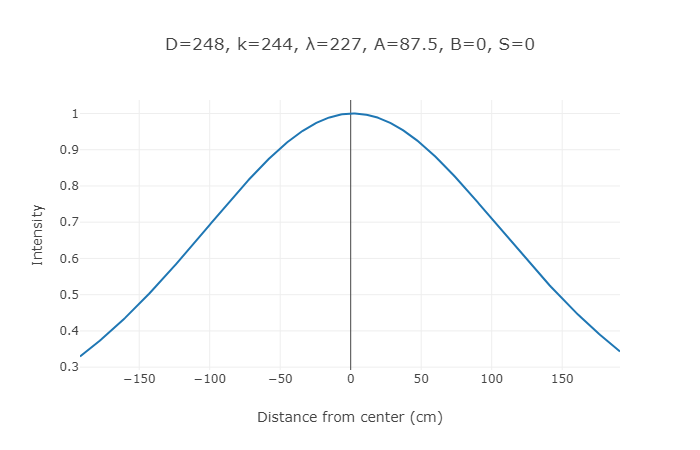
\includegraphics{diagrams/diffraction/single-slit-large-lambda.png}
\end{figure}

\begin{figure}[H]
    \caption{Double slit - Small wavelength}
    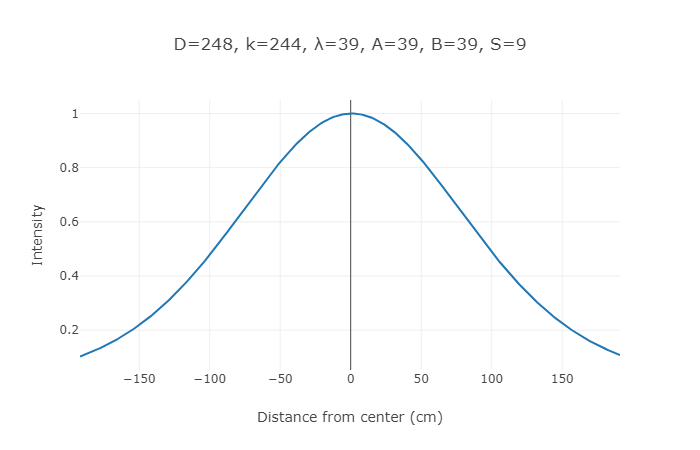
\includegraphics{diagrams/diffraction/double-slit-small-lambda.png}
\end{figure}

\begin{figure}[H]
    \caption{Double slit - Large wavelength}
    \includegraphics{diagrams/diffraction/double-slit-large-lambda.png}
\end{figure}

\begin{figure}[H]
    \caption{One slit twice as wide as the other - Large wavelength}
    \includegraphics{diagrams/diffraction/1-2-ratio-large-lambda.png}
\end{figure}

\pagebreak

\end{appendices}


\end{document}